% SPDX-License-Identifier: CC-BY-SA-4.0
%
% Copyright (c) 2021 Philipp Le
%
% Except where otherwise noted, this work is licensed under a
% Creative Commons Attribution-ShareAlike 4.0 License.
%
% Please find the full copy of the licence at:
% https://creativecommons.org/licenses/by-sa/4.0/legalcode

\chapter{Information and Coding Theory}

\begin{refsection}

Information exchange through a transmission channel is always subject to noise. Spread spectrum techniques can be used to harden the transmission against noise up a certain extent. However, noise and its disturbance on the information transmission cannot be completely avoided. ``Hardening against noise'' actually means: Reducing the probability of getting a wrongly decoded signal in the receiver.

As everything related to noise, statistics and probability are central terms. There is always a non-zero probability of modulating an erroneous signal. The probability increases as the \ac{SNR} decreases. A measure for the errors after signal demodulation is the \textbf{\acf{BER}} \index{bit error rate}, when binary symbols (bits) are transmitted. It is the ratio of the number of erroneously received bits $N_{err}$ divided by the number of totally transmitted bits $N_{tot}$.

\begin{equation}
	\mathrm{BER} = \frac{N_{err}}{N_{tot}}
\end{equation}
\nomenclature[S]{$\mathrm{BER}$}{Bit error rate}%

Even with a good \ac{SNR}, there is a small probability for receiving wrong bits and the \ac{BER} is greater than zero, even if close to zero. But, already one false bit may corrupt the communication, for example if a complex protocol is used in a higher layer of the \ac{OSI} stack.

In the chapter, techniques to deal with corrupt symbols will be discussed. By adding some redundancy, falsely demodulated symbols can be detected and even corrected. This ensures a reliable communication in the presence of noise. Even harsh condition with low \ac{SNR} can be mastered. Nowadays, the electromagnetic spectrum is used heavily by a huge number of services. Their signals may cause disturbances to each other (noise). Without error correction methods, it would be difficult to reliably communicate.

The basis for these symbol recovery techniques is proper \index{coding} \emph{coding}. \index{information and coding theory} \textbf{Information and coding theory} is the study of mathematical methods to describe information and their processing. Here, information are not considered as signals as in the chapters before -- information is now a discrete entity, which is the subject of mathematical analysis.

The applications of \emph{information and coding theory} are:
\begin{itemize}
	\item \textbf{Source coding}: Detecting and removing unnecessary redundancy in a stream of symbols. This also known as \emph{compression}.
	\item \textbf{Channel coding}: Adding systematically redundancy to a stream of symbols, in order to be able to detect and correct transmission errors in the receiver.
	\item \textbf{Cryptography}: Concealing the contents of the transmission to provide confidentiality.
	\item \textbf{Line coding}: Bringing the information into a representation, so that the transmission channel can transfer the information. (Not all signal representations of information can be transmitted equally, because they have different physical properties (bandwidth, etc.).) Actually, the line coding operates in the baseband. The line-coded baseband signal is than given to a mixer, which then produces the \ac{RF} signal for transmission over the channel.
\end{itemize}

% TODO: Maybe some line coding too
This chapter concerns with \emph{source coding} and \emph{channel coding}. They are the last missing part in our signal and information processing chain in a digital communication system.
\begin{itemize}
	\item Modulation brings the information onto a carrier which can be transmitted through a transmission channel.
	\item Spread spectrum and multiple access enabled sharing the transmission channel with different users.
	\item Source coding reduces the amount of data which must be transmitted (compression) and thereby improves the performance (data rate).
	\item Channel coding hardens the signal transmission against noise and disturbances. Erroneous symbols can be detected and corrected using mathematical methods.
\end{itemize}

% TODO: Figure showing the processing chain

It is important to note, that even channel coding cannot push the error probability or \ac{BER} down to exactly zero. A probability of decoding symbols wrongly is still there. However, channel coding significantly reduces this probability. The probability is so low, that it almost does not matter is reality. This is the criterion for a reliable communication.

\section{Information Model}

Information considered in a digital communication system is value-discrete. The information is represented by a set of symbols $x_i$ which is the \index{source alphabet} \emph{source alphabet} $\Omega$. Considering there are $M$ discrete symbols, the source alphabet is:

\begin{equation}
	\Omega = \bigcup\limits_{i = 1}^{M} x_i = \left\{x_1, x_2, \ldots, x_M\right\}
\end{equation}
\nomenclature[U]{$\bigcup\limits_{i = 1}^{M}$}{Union of sets}

All information originates from a source -- the information source in the Shannon-Weaver model. Here, it is called a \index{discrete information source} \emph{discrete information source}. The discrete information sources emits a series of discrete information (symbols) from the source alphabet $\Omega$. The series of symbols is then processed by further parts of the communication system -- coding, spreading, modulation, etc.

In this chapter, the actual content of the information is not important. The real interpretation of the symbols is a matter of the user of the communication system or higher layers in the \ac{OSI} stack, which is modelled as the discrete information source. Here, the information is just considered as symbols which are emitted by an abstract discrete information source.

\subsection{Memoryless Information Source}

A \index{message} \textbf{message} is a series of symbols out of the alphabet $\Omega$ which is emitted by a discrete information source. The message $\vec{m}$ has a length of $N_m$.
\begin{equation}
	\vec{m} = \left[x[0], x[1], \ldots, x[N_m-1]\right]
\end{equation}
$x[n] \in \Omega$ is a symbol of the source alphabet $\Omega$. $n$ is the index of the symbol in the message.

$x[n]$ can be any symbol\footnote{In the literature, \textbf{event} is used as a synonym, too. Here, we stick to \emph{symbol} to make the relationship to the symbols used for modulation and spreading clear.} $x_i \in \Omega$ out of the source alphabet. Now, the discrete information source is considered to be a black-box. It emits a series of symbols. But from the outside, a observer has no knowledge about the internals (like a algorithm which generates the symbols). So the symbol emission is random. The discrete information source is a random process. The emitted symbol $x[n]$ is a random variable.

In addition to the randomness of symbol emission, it is assumed that the source has no memory. That is, the emission of a symbol $x[n]$ does not depend on the past symbols $x[0], \ldots, x[n-1]$. So all samples (i.e. symbols) taken from the discrete information source are independent from each other. As a consequence, the discrete information source does not have an internal memory, which stores past symbols which upcoming symbols rely on. The source is a \index{discrete memoryless source} \textbf{discrete memoryless source}.

\begin{excursus}{Sources with memory}
	Of course, there are sources with a memory. Here, a emitted symbol depends on past symbols.
	
	An example is written English language. The symbols are the letters. The source alphabet comprises 26 letters. A random sequence of letters like ``qwubrfasdfnas'' does not make any sense. The letters in the sequence always depend on other letters to form words. Some letters like ``q'' furthermore only exist together with other letters (``qu'').
\end{excursus}

Each symbol $x_i$ has a certain probability $p_i$ of being emitted by the discrete information source. The occurence probabilities of all symbols must sum to $1$.

\begin{equation}
	\sum\limits_{i=1}^{M} p_i \stackrel{!}{=} 1
	\label{eq:ch08:dms_prob_sum}
\end{equation}

So a message $\vec{m}$ with a length of $N_m$ contains the symbol $x_i \in \Omega$ in average $N_m p_i$ times.

\begin{proof}{}
	The total length of the message $\vec{m}$ is the sum of the average number of occurences $N_m p_i$ of all $M$ symbols.
	\begin{equation}
		\begin{split}
			\dim \vec{m} &= \sum\limits_{i=1}^{M} N_m p_i \\
			 &= N_m \cdot \underbrace{\sum\limits_{i=1}^{M} p_i}_{= 1, \, \text{because of \eqref{eq:ch08:dms_prob_sum}}} \\
			 &= N_m
		\end{split}
	\end{equation}
	So the length of the message $\vec{m}$ is indeed $N_m$.
\end{proof}

A message where all symbols $x_i$ occur exactly $N_m p_i$ times is called a \textbf{typical sequence}. The position of the symbols $x_i$ are not fixed in the message. So, there are $N_{TS}$ possible combinations of typical sequences. The probability that a typical sequence of a certain combination is emitted is $P_{TS}$.
\begin{equation}
	P_{TS} = \prod\limits_{i = 1}^{M} p_i^{N_m p_i} = p_1^{N_m p_1} \cdot p_2^{N_m p_2} \cdot \ldots \cdot p_M^{N_m p_M}
	\label{eq:ch08:typseq_prob}
\end{equation}%
\nomenclature[Pts]{$P_{TS}$}{Probability that a typical sequence of a certain combination is emitted}%
According to Shannon, only typical sequences shall be considered, because all other sequences are very unlike to occur.
\begin{equation}
	\begin{split}
		N_{TS} \cdot P_{TS} &\stackrel{!}{=} 1 \\
		N_{TS} &= \frac{1}{P_{TS}} \\
		 &= \frac{1}{\prod\limits_{i = 1}^{M} p_i^{N_m p_i}}
	\end{split}
\end{equation}

\subsection{Information Content}

At this point, a \emph{discrete memoryless source} emits a sequence of symbols. The sequence of symbols -- the \emph{message} -- carries the \index{information} \textbf{information}. So the complete information is distributed over the symbols in the sequence.

Now considering each symbol $x_i \in \Omega$ independently, what is the contribution of that symbol $x_i$ to the information? A measure is the \index{information content} \textbf{information content} $\mathrm{I}(x_i)$ of the symbol $x_i \in \Omega$. \nomenclature[I]{$\mathrm{I}(x_i)$}{Information content of the symbol $x_i \in \Omega$}

The information content only depends on the probability of the symbol $p_i$, i.e. $\mathrm{I}(x_i)$ is a function of $p_i$.
\begin{equation}
	\mathrm{I}(x_i) = f(p_i)
\end{equation}
The function $f(\cdot)$ needs to be determined.

$\mathrm{I}(x_i)$ has some constraints.
\begin{itemize}
	\item If $p_i = 1$, then $\mathrm{I}(x_i) = 0$. $p_i = 1$ means that the source emits $x_i$ only. This makes the discrete memoryless source predictable. As a consequence, the message generated by this source does not contain any information -- the information content $\mathrm{I}(x_i)$ is zero. Remember that information leads to an increased knowledge in the receiver (Shannon-Weaver model in Chapter 1). A receiver cannot gain any knowledge from a predictable source, because it already has the knowledge ``there is only $x_i$''.
	\item Consequently, if $p_i < 1$, then $\mathrm{I}(x_i) > 0$.
\end{itemize}
Furthermore, $\mathrm{I}(x_i)$ must be non-negative.

\begin{example}{}
	The information content is some kind of measure of the worth a symbol. The higher the information content is, the more knowledge is gained in the receiver.
	
	Let's illustrate the worth: The information content $\mathrm{I}(x_i)$ is a function of the probability $p_i$ of the event (symbol) $x_i$.
	\begin{itemize}
		\item A very probable event is that a good friend is visiting you regularly for hanging-out. So you won't put much expense in tidy up your apartment.
		\item A less probable event is a visit by your grandparents. You want to make a good impression and clean every corner in your apartment. The expense is much higher.
	\end{itemize}
\end{example}

Let's define a event $C$ generated by the source. $C$ is a message composed of the symbols $x_1$ and $x_2$. So, $C$ is the intersection of $x_1$ and $x_2$.
\begin{equation}
	C = x_1 \cap x_2
\end{equation}

Because the symbols $x_1$ and $x_2$ are independent in a discrete memoryless source, the probability $\mathrm{P}(C)$ that the event $C$ occurs is:
\begin{equation}
	\mathrm{P}(C) = \mathrm{P}(x_1 \cap x_2) = \underbrace{\mathrm{P}(x_1)}_{= p_1} \cdot \underbrace{\mathrm{P}(x_2)}_{= p_2}
\end{equation}
where $\mathrm{P}(x_i)$ is an alternate notation for $p_i$.

The information content is additive. So, the information content of the event $C$ is the sum of the information contents of both symbols.
\begin{equation}
	\mathrm{I}(C) = \mathrm{I}(x_1) + \mathrm{I}(x_2)
	\label{eq:ch08:infocont_sum}
\end{equation}

Now, the function $f(\cdot)$ can be determined.
\begin{equation}
	\begin{split}
		\mathrm{I}(C) &= f\left(\mathrm{P}(C)\right) \\
		 &= f\left(\mathrm{P}(x_1 \cap x_2)\right) \\
		 &= f\left(\mathrm{P}(x_1) \cdot \mathrm{P}(x_2)\right)
	\end{split}
	\label{eq:ch08:infocont_prob}
\end{equation}

Setting \eqref{eq:ch08:infocont_sum} and \eqref{eq:ch08:infocont_prob} equal yields:
\begin{equation}
	\mathrm{I}(x_1) + \mathrm{I}(x_2) \stackrel{!}{=} f\left(\mathrm{P}(x_1) \cdot \mathrm{P}(x_2)\right)
	\label{eq:ch08:infocont_deriv1}
\end{equation}

A function which fulfils \eqref{eq:ch08:infocont_deriv1}, is:
\begin{equation}
	f(x) = K \log_{b} (x)
\end{equation}
Because $0 \leq p_i \leq 1$, the $\log_{b} (x)$ is always non-positive. So, the coefficient is $K < 0$.

The selection of parameters determines the unit of the information content. Usually, $K = -1$. The base $b$ can now be chosen:
\begin{itemize}
	\item $b = 2$: The unit is \si{bit}. Bit stands for \emph{binary digit} -- the two possible states for a Bit are 0 and 1.
	\item $b = e$ (natural logarithm): The unit is \si{nat}.
	\item $b = 10$: The unit is \si{hartley}.
\end{itemize}
The common practice is $b = 2$ and the unit of the information content is \si{bit}.

\begin{definition}{Information content}
	The \index{information content} \textbf{information content} $\mathrm{I}(x_i)$ of a symbol $x_i$ with a probability of $p_i$ is:
	\begin{equation}
		\mathrm{I}(x_i) = - \log_2 \left(p_i\right) = \log_2 \left(\frac{1}{p_i}\right)
		\label{eq:ch08:infocont}
	\end{equation}

	\textbf{The information content is a property of a symbol.}
\end{definition}

Now, imagine that a symbol $x_i \in \Omega$ should be encoded in a sequence of binary symbols (bits). How many bits are required to encode this symbol optimally? A ``more worthy symbol'' (low probability) requires more bits. A symbol with high probability should be encoded with fewer bits. The information content $\mathrm{I}(x_i)$ is a measure for the optimal number of bits.

The variable length encoding of symbols is the basis for compressing information (source coding). If more probable symbols are encoded with fewer bits, the total length of the encoded message is shorter, as if each symbol $x_i \in \Omega$ was encoded with the same number of bits.

\subsection{Shannon Entropy}

A discrete memoryless source emits a sequence of symbols. Each symbol has a information content defined by \eqref{eq:ch08:infocont}. Form this definition, the average information per emitted symbol can be determined.

What is the purpose? The average information per emitted symbol is a measure for the knowledge gain in the receiver, which a information source delivers.
\begin{itemize}
	\item If the information source is completely predictable (i.e. the emitted symbol sequence is already known by the receiver), no knowledge is gained by the receiver. The average information per emitted symbol is zero.
	\item If the receiver knows, that some symbols are more probable than others, it is no surprise that they are really received more often. However, there is a random process in the information source. The average information per emitted symbol is greater than zero.
	\item If the receiver is absolutely uncertain about which symbol is going to be emitted next, the average information per emitted symbol is at its maximum. This case is called \index{total surprise} \textbf{total surprise}.
\end{itemize}
The average information per emitted symbol is a measure for the uncertainty or surprise that a receiver of the information has.

The average information per emitted symbol $\mathrm{H}(X)$ is the expectation value of the information content $\mathrm{I}(x_i)$.
\begin{equation}
	\begin{split}
		\mathrm{H}(X) &= \E\left\{\mathrm{I}(x_i)\right\} \\
		 &= \sum\limits_{i=1}^{M} p_i \mathrm{I}(x_i) \\
		 &= - \sum\limits_{i=1}^{M} p_i \log_2 \left(p_i\right)
	\end{split}
\end{equation}

The average information per emitted symbol $\mathrm{H}(X)$ is called \index{information entropy} \textbf{information entropy}. The term ``entropy'' shows the relation to the Boltzmann-Gibbs formula of the entropy in thermodynamics. It is a probabilistic interpretation of the second principle of thermodynamics.
\begin{equation}
	S = - k \sum\limits_{i=1}^{M} p_i \log \left(p_i\right)
\end{equation}
where $k$ is the Boltzmann constant.

\begin{definition}{Information entropy}
	The \index{information entropy} \textbf{information entropy} $\mathrm{H}(X)$ of a information source which emits symbols $x_i \in \Omega$ (out of the source alphabet $\Omega$), where each symbol $x_i$ has a probability of $p_i$, is:
	\begin{equation}
		\mathrm{H}(X) = - \sum\limits_{i=1}^{M} p_i \log_2 \left(p_i\right)
		\label{eq:ch08:infoentropy}
	\end{equation}\nomenclature[H]{$\mathrm{H}(X)$}{Information entropy}

	\textbf{The information entropy is a property of a information source.}
\end{definition}

So the information entropy is the sum of the information contents of all possible symbols $x_i \in \Omega$ weighted by their probability $p_i$. This corresponds to a circumstance where all symbols occur exactly $N_m p_i$ times, which is a \emph{typical message} ($N_m$ is the message length). A \emph{typical message} has a probability $P_{TS}$ \eqref{eq:ch08:typseq_prob} of being emitted by the source. The information content of a \emph{typical message} is:
\begin{equation}
	\begin{split}
		\mathrm{I}_{TS} &= - \log_2 \left(P_{TS}\right) \\
		 &= - \log_2 \left(\prod\limits_{i = 1}^{M} p_i^{N_m p_i}\right) \\
		 &= - \sum_{i = 1}^{M} \log_2 \left(p_i^{N_m p_i}\right) \\
		 &= - N_m \sum_{i = 1}^{M} p_i \log_2 \left(p_i\right) \\
	\end{split}
\end{equation}
Now, the average information per emitted symbol in the message of length $N_m$ is
\begin{equation}
	\frac{\mathrm{I}_{TS}}{N_m} = - \sum_{i = 1}^{M} p_i \log_2 \left(p_i\right) = \mathrm{H}(X)
\end{equation}
which is the information entropy $\mathrm{H}(X)$. This shows an alternate derivation of the information entropy.

\begin{fact}
	For clarification:
	\begin{itemize}
		\item The information entropy is a property of a information source.
		\item The information content is a property of a symbol.
	\end{itemize}
\end{fact}

The maximum information entropy is called \index{decision quantity} \textbf{decision quantity} $\mathrm{D}(X)$.
\begin{equation}
	\mathrm{D}(X) = \max\limits_{p_i} \mathrm{H}(X)
\end{equation}
It can be shown that $\mathrm{D}(X)$ is achieved if all symbols $x_i$ are uniformly distributed and have equal probabilities:
\begin{equation}
	p_1 = p_2 = \ldots = p_M = \frac{1}{M}
\end{equation}
Consequently, the formula for the decision quantity can be derived.

\begin{definition}{Decision quantity}
	The \index{decision quantity} \textbf{decision quantity} $\mathrm{D}(X)$ of a information source which emits symbols $x_i \in \Omega$ (out of the source alphabet $\Omega$), where $\Omega$ comprises $M$ discrete symbols, is
	\begin{equation}
		\mathrm{D}(X) = \log_2 \left(M\right)
		\label{eq:ch08:dec_quant}
	\end{equation}
\end{definition}

\eqref{eq:ch08:dec_quant} is already known as a formula to determine how many bits are required to encode a symbol in bits. Let's say that a source emits symbols with 256 states (a byte). If all symbols have equal probability, the receiver has \emph{total surprise} and the information entropy is at its maximum. The number of bits required to encode one byte is $\log_2 \left(256\right) = \SI{8}{bit}$.

\begin{example}{Coin toss}
	Consider you toss a coin. The coin lands on heads with a probability of $p$ and lands on tails with a probability of $1-p$. The question is: How many bits do you need in average to describe the output of the coin toss?
	\begin{itemize}
		\item If $p=0$ (always lands on heads) or $p=1$ (always lands on tails), the coin toss is predictable and does not give any information. So the information entropy is zero.
		\item For $p=0.5$ (equal probability of head and tail), the surprise is total. The information entropy is at its maximum.
	\end{itemize}
	The information entropy is the measure to describe the required number of bits in average.
	\begin{equation}
		\begin{split}
			\mathrm{H}(X) &= - \sum\limits_{i=1}^{M} p_i \log_2 \left(p_i\right) \\
			 &= - p \log_2 \left(p\right) - \left(1-p\right) \log_2 \left(1-p\right)
		\end{split}
	\end{equation}
	
	A graphical representation is:
	\begin{figure}[H]
		\centering
		\begin{tikzpicture}
			\begin{axis}[
				height={0.3\textheight},
				width=0.6\linewidth,
				scale only axis,
				xlabel={$p$},
				ylabel={$\mathrm{H}(X)$},
				%grid style={line width=.6pt, color=lightgray},
				%grid=both,
				grid=none,
				legend pos=outer north east,
				axis y line=middle,
				axis x line=middle,
				every axis x label/.style={
					at={(ticklabel* cs:1.05)},
					anchor=north,
				},
				every axis y label/.style={
					at={(ticklabel* cs:1.05)},
					anchor=east,
				},
				xmin=0,
				xmax=1.2,
				ymin=0,
				ymax=1.2,
			]
				\addplot[blue, smooth, domain=0.01:0.99, samples=50] plot(\x, {-\x*log2(\x) - (1-\x)*log2(1-\x)});
			\end{axis}
		\end{tikzpicture}
		\caption{Entropy of a coin toss depending on the probability of a certain event}
	\end{figure}

	The decision quantity (maximum information entropy) is \SI{1}{bit}. If $p$ is different from $0$, $0.5$ or $1$, a value of less than \SI{1}{bit} is required to encode the output of the coin toss -- the output tends to be more head or more tail, so it is more predictable.
\end{example}

\subsection{Source Efficiency}

If the discrete memoryless source delivers a total surprise, it yields the maximum gain of knowledge in the receiver. So, it is most efficient at this point.

An information source with a lower information entropy, is less efficient. It can be said, that the source delivers partly redundant information, because its surprise is not total anymore.

The \index{absolute redundancy} \textbf{absolute redundancy} is:
\begin{equation}
	R_X = \mathrm{D}(X) - \mathrm{H}(X)
\end{equation}

The \index{relative redundancy} \textbf{relative redundancy} is referenced to the maximum entropy:
\begin{equation}
	\rho_X = \frac{R_X}{\mathrm{D}(X)} = 1 - \frac{\mathrm{H}(X)}{\mathrm{D}(X)}
\end{equation}

$1 - \rho_X$ is the \emph{source efficiency}.

\begin{definition}{Source efficiency}
	The \index{source efficiency} \textbf{source efficiency} is:
	\begin{equation}
		\eta_X = \frac{\mathrm{H}(X)}{\mathrm{D}(X)}
	\end{equation}
\end{definition}

\section{Source Coding}

Generally, the information emitted by source cannot be directly sent over the transmission channel. The transmission channel has another alphabet than the source alphabet. Thus, an adaption from the source to the channel is required.

\begin{itemize}
	\item An \index{information representing code} \textbf{information representing code} is a processable form of the information in the communication system. Whereas information is a abstract term, coded information does really exist as a digital or analogue signal.
	\item The coding of the source information must be as efficient as possible. More probable information must be encoded with shorter codes than less probable information. This saves transmission time and storage space for the information. The technique behind this coding is called \index{compression} \textbf{compression} or \index{source coding} \textbf{source coding}.
\end{itemize}

\index{coding} \textbf{Coding} is a bijective (reversible) mapping between two alphabets $\Omega_1$ and $\Omega_2$. The probability of the corresponding symbols in both alphabets is equal. $\Omega_1$ can be seen as the \emph{source alphabet}. $\Omega_2$ contains the \index{codewords} \textbf{codewords} (of the \emph{information representing code}).

For now, we assume \emph{noiseless channels}. That is, the symbols sent over the transmission channel are not affected by noise. The receiver gets exactly the same symbols as sent by the transmitter.

\subsection{Information Representing Code}

The \emph{codewords} must be viewed as abstract symbols. They can actually have different lengths like in the following example:
\begin{equation}
	\Omega = \left\{x_1, x_2, x_3, x_4\right\} = \left\{\left(0\right)_2, \left(10\right)_2, \left(110\right)_2, \left(111\right)_2\right\}
\end{equation}
The symbols of $\Omega$ consist of binary symbol sequences with varying length. So, a binary symbol stream of $\left(011010111\right)_2$ is actually the symbol sequence $x_1, x_3, x_2, x_4$. The binary representation can really exist as a digital or analogue signal and can therefore be processed. It is an \emph{information representing code}.

The mapping of the above example is:
\begin{table}[H]
	\centering
	\caption{Code mapping example}
	\begin{tabular}{|l|l|}
		\hline
		Symbol from $\Omega_1$ & Symbol from $\Omega_2$ \\
		\hline
		\hline
		$x_1$ & $\left(0\right)_2$ \\
		\hline
		$x_2$ & $\left(10\right)_2$ \\
		\hline
		$x_3$ & $\left(110\right)_2$ \\
		\hline
		$x_4$ & $\left(111\right)_2$ \\
		\hline
	\end{tabular}
\end{table}

The \index{information representing code} \textbf{information representing code} is a kind of carrier for the information. The code enables the existence of the information in physical or logical form.

The binary code is the most common representation for information in a digital communication system. However, there are other examples of \emph{information representing codes}:
\begin{itemize}
	\item The Morse code encodes letters by transmitting a short (dot) or long (dash) tone. The length of Morse code symbols is variable. More common letters in the English language (high probability) have a shorter symbol than less common letters. This significantly speeds up the transmission of letters.
	\item \ac{PCM} is used to encode discrete-values of a sampled signal (see Chapter 4). Each symbol represents a discrete value.
\end{itemize}

\begin{excursus}{Coding in biology}
	Codes can be found everywhere. An example is the genetic code of living organisms. Organisms are composed of proteins. Their building plan is stored in the \ac{DNA} of the cells. The production of a protein follows certain steps:
	\begin{itemize}
		\item The \ac{DNA} is trans-scripted. The protein building plan (the genetic information) is encoded in \ac{mRNA}.
		\item The \ac{mRNA} is sent to the ribosomes of the cell. They decode the \ac{mRNA} and produce \ac{tRNA}.
		\item The \ac{tRNA} then is converted into a protein.
	\end{itemize}
	The genetic code is represented by either \ac{DNA} or \ac{RNA}. They carry the genetic information.
\end{excursus}

\subsection{Code Efficiency}

Information representing code can have a varying length. Let's define the \emph{lengths of codewords}. The length of the codeword $c_i$ is $N_{c,i}$. $c_i$ is mapped to $x_i$ from the source alphabet.

The probability of $c_i$ equals the probability of $x_i$.
\begin{equation}
	\mathrm{P}\left(c_i\right) = \mathrm{P}\left(x_i\right) = p_i
\end{equation}

The \emph{average length of codewords} $\overline{N_c}$ is:
\begin{equation}
	\overline{N_c} = \sum\limits_{i=1}^{M} p_i N_{c,i}
\end{equation}

Each codeword consists of letters $l_j \in L$ from a alphabet $L$. A binary alphabet is the set of $M_L = 2$ letters $L = \left\{0, 1\right\}$. The codewords $c_i$ are groups of $N_{c,i}$ letters $l_j \in L$.

The final encoded symbol stream only consists of the letters $l_j \in L$. For an outside observer, it seems that the letters $l_j$ are emitted randomly. The information entropy is $\mathrm{H}\left(L\right)$.

The information entropy is connected to the information entropy of the source $\mathrm{H}\left(X\right)$. This is the \emph{entropic compression relation}.
\begin{equation}
	\mathrm{H}\left(X\right) = \overline{N_c} \cdot \mathrm{H}\left(L\right)
\end{equation}
Because of the same symbol probabilities, both information entropies of the source $\mathrm{H}\left(X\right)$ and codewords $\mathrm{H}\left(C\right)$ are equal.

If the coding is optimal, the letters are emitted with total surprise. Thus, the information entropy for $L$ is at maximum:
\begin{equation}
	\mathrm{D}\left(L\right) = \log_2 \left(M_L\right)
\end{equation}
Thus, the optimal (minimal) average length of codewords $\overline{N_{c,min}}$ is:
\begin{equation}
	\overline{N_{c,min}} = \frac{\mathrm{H}\left(X\right)}{\mathrm{D}\left(L\right)} = \frac{\mathrm{H}\left(X\right)}{\log_2 \left(M_L\right)}
\end{equation}
For the optimal (minimal) average length of codewords $\overline{N_{c,min}}$, the costs for the transmission is lowest (highest speed, lowest storage size).

\begin{definition}{Code efficiency}
	The \index{code efficiency} \textbf{code efficiency} is the ratio of the minimal average length of codewords $\overline{N_{c,min}}$ and the average length of codewords of the current coding $\overline{N_c}$.
	\begin{equation}
		\eta_C = \frac{\overline{N_{c,min}}}{\overline{N_c}} = \frac{\mathrm{H}\left(X\right)}{\overline{N_c} \cdot \log_2 \left(M_L\right)}
	\end{equation}
\end{definition}

If the code efficiency is $\eta_C = 1$, i.e. $\overline{N_c} = \overline{N_{c,min}}$, the code is an \index{absolute optimal code} \textbf{absolute optimal code}. For an absolute optimal code, the source coding (compression) does not have any effect, because the code is already optimal.

\subsection{Compression Algorithms}

Compression is the act of re-encoding data so that the it requires less symbols to describe the data. That is, the output alphabet has a higher code efficiency.

There are two types of compression:
\begin{itemize}
	\item \textbf{Lossless compression} -- The data is preserved. It is only re-encoded. The original symbols from the input alphabet can be restored.
	\item \textbf{Lossy compression} -- The original data cannot be restored. Generally, only irrelevant parts of data are remove. The receiver is still able to gain knowledge from the information transferred. However a full recovery of data is not possible.
\end{itemize}

Examples for lossless compression algorithms are ``Deflate algorithms'' in ZIP, RAR, GZip, BZip2 or LZMA archives. These archives are files which contain other files on a computer file system. The files are compressed. Their size is reduced by a proper algorithm -- so they are ``deflated''. The original files can be restored with a reverse algorithm (``inflating''). The input alphabet is a symbol sequence with uniform length -- 1 byte consisting of 8 bits. The output alphabet uses variable length symbol sequences.

Examples for lossy compression algorithms are the encodings used for image, audio and video files on a computer (images: JPEG, PNG; audio: MPEG-3/mp3; video: MPEG-4/mp4, ...). The original data stream from the audio or video sensor is heavily compressed. The compression algorithm only uses approximations of the original data, so it cannot be fully reconstructed afterwards. However, humans senses certainly will not note any difference. Furthermore, the compression can be so heavy that the receiver notices a lack in quality, but is still able to get the information transported. In return, the data size is even more reduced.

Especially lossy algorithms are commonly used to encode audio and video streams in digital communication systems. With a variable compression ratio, the data rate can be adapted to the capacity of the transmission channel which relies on the noise conditions. The information receiver will experience a drop in quality if the data rate is reduced. However, the communication is still possible, because the receiver still gains knowledge.

\subsection{Example: Shannon-Fano Binary Coding}

The \index{Shannon-Fano algorithm} Shannon-Fano algorithm is a lossless compression algorithm. It is efficient, but it is proven that it does not deliver the best encoding for any kind of source. The Huffman algorithm, which was invented later, yields optimal encoding.

The Shannon-Fano algorithm uses the circumstance that symbols have a different probability of occurence. Symbols with higher probability are encoded with shorter symbol sequences. Symbols with lower probability use longer symbol sequences in the output.

The steps are:
\begin{enumerate}
	\item Preparation:
	\begin{enumerate}
		\item Determine the occurence probability of every symbol in the input source alphabet.
		\item Sort the symbols by their occurence probability in descending order.
	\end{enumerate}
	\item Partitioning:
	\begin{enumerate}
		\item Assign the sorted symbols into two partitions $S_0$ and $S_1$ of same or almost equal probability.
		\item In each partition $S_0$ and $S_1$, divide the symbols into two partitions $S_{00}$ and $S_{01}$ or $S_{10}$ and $S_{11}$, respectively, of same or almost equal probability, again.
		\item Repeat until each partition only has one symbol from the input source alphabet.
	\end{enumerate}
	\item Output symbols (codewords) assignment:
	\begin{enumerate}
		\item Assign the symbol $0$ to the first partition $S_0$ and the symbol $1$ to the second partition $S_1$.
		\item In each sub-partition, extend the output symbol by $0$ for the first sub-sub-partition $S_x0$ and by $1$ for the second sub-sub-partition $S_x1$.
		\item Repeat until all partitions have an output symbol assigned.
	\end{enumerate}
\end{enumerate}

\begin{example}{Shannon-Fano binary coding of a discrete memory less source}
	A input source alphabet has the symbols $s_1 = (00)_2$, $s_2 = (01)_2$, $s_3 = (10)_2$ and $s_4 = (11)_2$ with the following probabilities:
	\begin{table}[H]
		\centering
		\begin{tabular}{|l|l|l|l|l|}
			\hline
			Symbol & $s_1$ & $s_2$ & $s_3$ & $s_4$ \\
			\hline
			Sequence & $(00)_2$ & $(01)_2$ & $(10)_2$ & $(11)_2$ \\
			\hline
			Probability & $0.5$ & $0.25$ & $0.125$ & $0.125$ \\
			\hline
		\end{tabular}
	\end{table}

	The partitions and codewords are:
	\begin{table}[H]
		\centering
		\begin{tabular}{|l|l|l|l|l|l|}
			\hline
			Symbol & Probability & \multicolumn{3}{l|}{Partitions} & Codeword \\
			\hline
			\hline
			$s_1 = (00)_2$ & $0.5$ & \multicolumn{3}{l|}{$S_0$} & $(0)_2$ \\
			\hline
			$s_2 = (01)_2$ & $0.25$ & \multirow{3}{*}{$S_1$} & \multicolumn{2}{l|}{$S_{10}$} & $(10)_2$ \\
			\cline{1-2}\cline{4-6}
			$s_3 = (10)_2$ & $0.125$ & & \multirow{2}{*}{$S_{11}$} & $S_{110}$ & $(110)_2$ \\
			\cline{1-2}\cline{5-6}
			$s_4 = (11)_2$ & $0.125$ & & & $S_{111}$ & $(111)_2$ \\
			\hline
		\end{tabular}
	\end{table}

	The most probable symbol $s_1 = (00)_2$ is encoded by a codeword $c_1 = (0)_2$ of length 1. The least probable symbols $s_3 = (10)_2$ and $s_4 = (11)_2$ are encoded by codewords of length 3.
	
	So, the input sequence $(0010010011010000)_2 = [(00)_2, (10)_2, (01)_2, (00)_2, (11)_2, (01)_2, (00)_2, (00)_2]$ (length 16) would be encoded to $(01101001111000)_2 = [(0)_2, (110)_2, (10)_2, (0)_2, (111)_2, (10)_2, (0)_2, (0)_2]$ (length 14). 2 bits could be saved.
\end{example}

\section{Channel Coding}

Generally, the bit error probability is low for good \ac{SNR}, and vice versa. However, the bit error probability is never zero. Thus even for good \ac{SNR} (low noise conditions), there is a non-zero probability of bit errors.

Single bit errors can significantly affect the communication. Higher protocol layers in the \ac{OSI} stack cannot decode the information and whole packets (consisting of several hundrets to thousands bits) are lost.

It is important to keep in mind, that every transmission channel is noisy. So, all real digital communication is subject to noise and bit errors. As a consequence, there is a great need of coping with bit errors in order to establish a reliable communication channel.

\index{Channel coding} \emph{Channel coding} provides a countermeasure to detect and even correct bit errors. Whereas \emph{source} aimed to remove redundancies in data, channel coding systematically adds redundancy. This redundancy is derived from the input symbol sequence. If symbols are corrupted by noise, the redundant symbols are used to discover the corruption and recover the errors -- both to some extend.

In modern high data rate, digital communication systems, channel coding is essential. Noise and interference from other users are present in most circumstances. So communication equipment must always some extend of protection.

\subsection{Channel Capacity and Bit Errors}

The transmission can be described by two alphabets -- the source alphabet $X$ and the alphabet of received symbols $Y$. The transmission channel maps the symbols $x_i \in X$ to symbols from $y_j \in Y$.

% TODO: Mapping figure

Both alphabets $X$ and $Y$ have probabilities for their symbols $\mathrm{P}(x_i) = p_{X,i}$ or $\mathrm{P}(y_j) = p_{Y,j}$, respectively. The transmission through the transmission channel can be described by the joint distribution $\mathrm{P}(y_j/x_i) = p_{Y/X,j,i}$, that is, the probability of receiving a symbol $y_j$ if $x_i$ was transmitted.

The joint probabilities can be arranged in the joint probability matrix $\mat{P}_{Y/X}$. The dimension is $N_Y \times N_X$, where $N_X$ is the number of symbols in $X$ and $N_Y$ is the number of symbols in $Y$.

\begin{equation}
	\mat{P}_{Y/X} = \left[\begin{matrix}
		p_{Y/X,1,1} & p_{Y/X,2,1} & \ldots & p_{Y/X,N_Y,1} \\
		p_{Y/X,1,2} & p_{Y/X,2,2} & \ldots & p_{Y/X,N_Y,2} \\
		\vdots & \vdots & \ddots & \vdots \\
		p_{Y/X,1,N_X} & p_{Y/X,2,N_X} & \ldots & p_{Y/X,N_Y,N_X} \\
	\end{matrix}\right]
\end{equation}

For each transmitted symbol $x_i$, one of the symbols $y_j$ must be received. So the probabilities in each row of $\mat{P}_{Y/X}$ must sum up to $1$.

\begin{equation}
	\sum\limits_{j = 1}^{N_Y} p_{Y/X,j,i} = 1 \qquad \forall 1 \leq i \leq N_X
\end{equation}

Under ideal conditions, $X$ and $Y$ have the same number of symbols (i.e. $N_X = N_Y$) and $x_i$ maps to $y_j$ with $i = j$. So, $p_{Y/X,j,i} = 1$ for $i = j$ and $p_{Y/X,j,i} = 0$ for $i \neq j$. These ideal conditions assume a noise-free environment. With presence of noise, there is a non-zero probability $p_{Y/X,j,i} > 0, i \neq j$ of receiving a wrong symbol -- a different symbol than the one which has been transmitted.

A measure for the dependence of the two random variables $X$ and $Y$ is the \index{mutual information} \textbf{mutual information}. It quantifies the amount of information $Y$ gained by the receiver by observing another random variable $X$, which is the transmitter output.

\begin{definition}{Mutual information}
	The \index{mutual information} \textbf{mutual information} of two jointly discrete random variables $X$ and $Y$ is:
	\begin{equation}
		\mathrm{I}\left(X; Y\right) = \sum\limits_{j = 1}^{N_Y} \sum\limits_{i = 1}^{N_X} p_{Y/X,j,i} \cdot \log_2 \left(\frac{p_{Y/X,j,i}}{p_{X,i} \cdot p_{Y,j}}\right)
	\end{equation}%
	\nomenclature[I]{$\mathrm{I}\left(X; Y\right)$}{Mutual information between $X$ and $Y$}
	
	The mutual information is a measure for \emph{how many bits are delivered per symbol}.
\end{definition}

If $X$ and $Y$ are totally independent from each other, the mutual information will be zero. The total independence describes noise and noise does not lead to an information gain in the receiver. If the dependence between $X$ and $Y$ is greater, the mutual information will be higher, indicating a grater information gain in the receiver.

There is an upper bound for the amount of information which can be reliably transmitted over a transmission channel. Source $X_0$ which optimally encodes the symbols delivers the best achievable information gain at the receiver. This upper limit is the \index{channel capacity} \textbf{channel capacity}.

\begin{definition}{Channel capacity}
	The \index{channel capacity} \textbf{channel capacity} $C$ is the upper limit of mutual information.
	\begin{equation}
		C = \max\limits_{p_{X,i} \rightarrow p_{X_0,i}} \mathrm{I}\left(X; Y\right)
	\end{equation}
\end{definition}

Now, the mutual information $\mathrm{I}\left(X; Y\right)$ of a source $X$ can be related to the optimum of source $X_0$.

\begin{definition}{Channel efficiency}
	The \index{channel efficiency} \textbf{channel efficiency} is the ratio of the mutual information to the theoretical optimum.
	\begin{equation}
		\eta_C = \frac{\mathrm{I}\left(X; Y\right)}{C}
	\end{equation}
\end{definition}

% For a digital communication system, the symbol sets are $X = \left\{0, 1\right\}$ and $Y = \left\{0, 1\right\}$. The probabilities of receiving a wrong symbol are $p_{Y/X,2,1}$ and $p_{Y/X,1,2}$

By dividing the \emph{channel capacity} by the symbol period $T_{sym}$, the maximum \index{information rate} \textbf{information rate} is obtained.

\begin{definition}{Information rate}
	The \index{information rate} \textbf{information rate} is the number of bits per second.
	\begin{equation}
		I_t = \frac{\mathrm{I}\left(X; Y\right)}{T_{sym}}
	\end{equation}

	The upper bound -- the maximum information rate -- is at maximum channel capacity.
	\begin{equation}
		C_t = \frac{C}{T_{sym}}
	\end{equation}
\end{definition}

As proven by Shannon and Hartley, the upper bound of the information rate is related to
\begin{itemize}
	\item the noise conditions -- namely the \ac{SNR} and
	\item the signal bandwidth.
\end{itemize}

\begin{definition}{Shannon-Hartley theorem}
	\begin{equation}
		C_t = B \cdot \log_2 \left(1 + \frac{P_S}{P_N}\right)
	\end{equation}
	where
	\begin{itemize}
		\item $B$ is the signal bandwidth,
		\item $P_S$ is the signal power and
		\item $P_N$ is the noise power.
	\end{itemize}
\end{definition}

Please note, that $P_S/P_N$ is the \ac{SNR}.

As consequences,
\begin{itemize}
	\item More information can be reliably transferred, if the bandwidth is larger.
	\item More information can be reliably transferred, if the \ac{SNR} is better.
\end{itemize}

% TODO: Bit error

\subsection{Error Control Strategies}

Every real transmission channel is noisy and has a non-zero probability of bit errors. So, a digital communication system should be able to detect errors. This ensures a reliable communication. Erroneous messages with wrong bits are detected and rejected. However, the data must be recovered. Common approaches to accomplish this are:
\begin{itemize}
	\item \acf{ARQ} -- The error is detected by the receiver. It then requests a re-transmission of the message from the sender. The request is issued automatically by some logic in the receiver. The user will not notice the presence of the error, because only re-transmitted and correct data is send to higher layers in the \ac{OSI} stack. However, the net data rate will decrease. The re-transmission requires additional transmission time which cannot be used to transmit other data.
	\item \acf{FEC} -- Using mathematical methods, errors be corrected in addition to detecting them. The error correction is only possible until a certain extend. But usually the bit error probability is relatively low in good \ac{SNR} conditions. So the capability of correcting only a couple of bit errors in a message is enough. The advantage of \ac{FEC} compared to \ac{ARQ} is that no re-transmission is required and the transmission channel is used more effectively.
	\item Stop and wait -- Sender and receiver communicate over a half- or full-duplex channel. If the receiver detects no error in the message it sends an \ac{ACK} indication back to the sender. The sender then sends the next message. If the receiver detects an error, it sends a \ac{NAK} back to the sender. The sender repeats the transmission of the message until it receives an \ac{ACK}. The described mechanism is also called \emph{flow control}.
\end{itemize}

Especially \ac{ARQ} and \ac{FEC} can be combined in an hybrid-\acs{ARQ}-\acs{FEC} system. This the advantages of both saving transmission time on the channel and the ability of re-transmitting messages in harsh \ac{SNR} conditions.

Even though, error control strategies provide strong countermeasures against bit errors, there is still a small remaining probability of remaining errors which
\begin{itemize}
	\item are not detected or
	\item are detected, but wrongly corrected.
\end{itemize}

\emph{Channel coding} is required to detect errors. Using eligible coding, error correction is possible, too. Let's have closer look at these coding mechanisms.

\subsection{Types of Error Control Codes}

Coding source symbols produces codewords. The rules for producing these codewords are called \index{code} \textbf{code}. They can be classified using the many criteria. The following list shows an excerpt:

\begin{itemize}
	\item Processing strategy:
	\begin{itemize}
		\item \index{block code} \textbf{Block codes} -- The information is arranged in blocks of $k$ bits. $q$ control bits are added, forming a codeword of length $n$.
		\item \index{convolutional code} \index{continuous code} \textbf{Continuous (convolutional) code} -- The information is precessed as a stream.
	\end{itemize}
	\item Possibility of reading the information in clear from the codeword:
	\begin{itemize}
		\item \index{systematic code} \textbf{Systematic code} -- The information can be read in clear from the codeword. The control bits are just added. The original information is left intact. An advantage is that the receiver can omit the decoding stage, with the drawback of loosing error detection and correction capability, but with the advantage of reducing complexity.
		\item \textbf{Non-systematic code} -- Information and control bits cannot be read in clear. A decoder is always required in the receiver.
	\end{itemize}
\end{itemize}

\subsection{Detection and Error Correcting Block Codes}

Error detection and correction is only possible if redundancy is added. That is, additional bits are added to the message.

Assume that the information is $k$ bits long. $q$ bits are added by the channel coding to provide error detection and correction. The total message is $n = k + q$ bits long. The $q$ bits are the \emph{parity bits} and add redundancy.

\begin{itemize}
	\item $k$ information bits
	\item $q$ parity or control bits
	\item $n = k + q$ message bits
\end{itemize}

The $n$ bits of the message now form the \emph{codeword}. The $q$ parity bits are dependent on the $k$ information bits. This fact restricts all theoretically possible $2^n$ codewords to a subset $2^k$ codewords.

\paragraph{Notation.}

The parameters of a block code are written in the form $(n, k)_b$. The index $b$ denotes the number of symbols in the codeword alphabet (not source alphabet). For binary codes using bits it is $b = 2$ and can be omitted. So a $(63, 57)$ code means: $n = 63$ message bits ($b = 2$), $k = 57$ information bits and $q = n - k = 6$ parity bits. 

\paragraph{Hamming distance.}

An important measure to analyse codewords is the \index{hamming distance} \textbf{hamming distance}.

\begin{definition}{Hamming distance}
	The \index{hamming distance} \textbf{hamming distance} $\mathrm{d}\left(\vec{v}_i, \vec{v}_j\right)$ is the number of positions for which two codewords $\vec{v}_i$ and $\vec{v}_j$ differ.
	\begin{equation}
		\mathrm{d}\left(\vec{v}_i, \vec{v}_j\right) = \sum\limits_{k=1}^{n} \vec{v}_i \bigoplus \vec{v}_j
	\end{equation}
	\nomenclature[d]{$\mathrm{d}\left(\vec{v}_i, \vec{v}_j\right)$}{Hamming distance between codewords $\vec{v}_i$ and $\vec{v}_j$}
\end{definition}

$\bigoplus$ denotes a bitwise \ac{XOR} operation. If two codewords are equal the hamming distance is $\mathrm{d}\left(\vec{v}_i, \vec{v}_i\right) = 0$.

\begin{example}{Hamming distance}
	The hamming distance of the codewords
	\begin{itemize}
		\item $\vec{v}_1 = \left[1, 0, 0, 1, 0, 1, 1, 0\right]$ and
		\item $\vec{v}_2 = \left[1, 0, 1, 0, 1, 0, 1, 1\right]$
	\end{itemize}
	is $\mathrm{d}\left(\vec{v}_1, \vec{v}_2\right) = 5$.
\end{example}

\paragraph{Hamming space.}

A codewords with $n$ bits has $2^n$ possible combinations. If there is a bit error, the codeword is changed into another one. This situation must be coped with.

The idea behind channel coding is that only $2^k$ out of the $2^n$ codewords are valid. The valid codewords are selected systematically. All valid codewords have a \emph{hamming distance} of $d_{min}$.
\begin{equation}
	d_{min} = n - k + 1
	\label{eq:ch08:hamming_dist_code}
\end{equation}
As a consequence, if there is a bit error. The resulting codewords is invalid because it is not one of the $2^k$ valid ones. This means that up $d_{min} - 1$ bit errors can be detected.

\begin{fact}
	Up to $d_{min} - 1$ bit errors can be detected, where $d_{min}$ is the \emph{hamming distance} between the valid codewords.
\end{fact}

All $2^n$ possible (but not necessarily valid) codewords span an $n$-dimensional space -- the \index{hamming space} \textbf{hamming space}. It is the set $W$ of all codewords. The valid codewords form a \emph{linear subset} $V$. The condition of $V$ is $\mathrm{d}\left(\vec{v}_i, \vec{v}_j\right) \geq d_{min} \forall \vec{v}_i \in V, \vec{v}_j \in V, i \neq j$. Another condition for the \emph{linear subset} $V$ is that the codeword $v_0 = 00\ldots0$ (all bits zero) is element of the set $V$ -- $v_0 \in V$.

\begin{example}{Hamming space and error detecting codes}
	The hamming space has a dimension of $n = 3$. There are the possible codewords $W$.
	\begin{equation}
		W = \left\{\begin{matrix}
			\mathbf{000}\\
			001\\
			010\\
			\mathbf{011}\\
			100\\
			\mathbf{101}\\
			\mathbf{110}\\
			111
		\end{matrix}\right\}
	\end{equation}
	
	Now, $k = 2$. All four valid codewords in $V$ are marked bold in the upper equation. Keep in mind that $000$ must be always part of $V$ -- because $V$ is a linear subset.
	\begin{equation}
		V = \left\{\begin{matrix}
			000\\
			011\\
			101\\
			110
		\end{matrix}\right\}
	\end{equation}
	The hamming distance between all valid codewords is $d_{min} = n - k + 1 = 2$.

	The source alphabet $\Omega$ of message now comprises $2^k = 4$ possible symbols:
	\begin{equation}
		\Omega = \left\{00, 01, 10, 11\right\}
	\end{equation}

	Now the symbols from the source alphabet are mapped to the valid codewords:
	\begin{table}[H]
		\centering
		\begin{tabular}{|l|l|}
			\hline
			Symbol & Codeword \\
			\hline
			\hline
			$00$ & $\mathbf{00}0$ \\
			\hline
			$01$ & $\mathbf{01}1$ \\
			\hline
			$10$ & $\mathbf{10}1$ \\
			\hline
			$11$ & $\mathbf{11}0$ \\
			\hline
		\end{tabular}
	\end{table}
	The first bits in the codewords are marked bold. They resemble the bits in the original symbol. The original symbol has a length of $k$ bits (information bits). Then $q = 1$ bit is added (parity bit). They form the codeword of length $n = k + q$ (message bits). \textbf{The code is systematic.} The message can be read directly from the codeword.
	
	There is a simple rule, for the parity bit. The number of all ones in the codeword must be even. This is fulfilled for all valid code words.
	
	Up to $d_{min} - 1 = 1$ bit errors can be detected. For example, if a symbol $01$ shall be transmitted, it is mapped to the codeword $011$. If there is one bit error, the receiver may get a $001$. The receiver now detects that this received codeword is invalid because the number of ones is not even (and the codeword is not part of $V$). The error was successfully detected.
	
	Of course, if there are two bit errors, the resulting codeword would be valid, although it is wrong. This is a case of non-detectable errors. They are less likely than one-bit errors. However, in poor \ac{SNR} conditions they can occur. Higher values of $q$ must be used. $k$ is thereby reduces -- less symbols can be encoded in the codewords. But the transmission is more robust.
\end{example}

\paragraph{Maximum Likelihood Decoding}

In addition to the $d_{min} - 1$ detectable bit errors, it is even possible to correct bit errors up to a certain extend. Let's assume that
\begin{itemize}
	\item the code has a hamming distance of $d_{min} > 2$ and
	\item the probability of more than one bit error is very low.
\end{itemize}
If a codeword with one bit error is received, it
\begin{itemize}
	\item is invalid (not part of $V$),
	\item but is is close to a valid codeword. The hamming distance to the next valid codeword is $1$. Because the valid codewords have a hamming distance of $d_{min} > 2$, the hamming distance between the invalid, received codewords and all other valid codewords is greater $1$.
\end{itemize}
As a consequence, the invalid, received codeword can be assigned to the valid codeword with hamming distance $1$. The probability that it was the originally transmitted codeword is high, because more than one bit errors are very unlikely.

In more formal way, the detected codeword $\tilde{y}$ is the codeword which has maximum likelihood to the actually received codeword $y$. $\tilde{y}$ is then assumed to have been transmitted by the source as $x$.
\begin{equation}
	\tilde{y} = \argmax\limits_{x \in V} L(x, y)
\end{equation}
The likelihood is determined by the likelihood function $L(x, y)$. The likelihood for the codewords $x$ and $y$ is inverse proportional to their hamming distance.
\begin{equation}
	L(x, y) \propto \frac{1}{\mathrm{d}\left(x, y\right)}
\end{equation}
As a consequence, the \index{maximum likelihood decoding} \textbf{maximum likelihood decoding} can be reformulated as:
\begin{equation}
	\tilde{y} = \argmin\limits_{x \in V} \mathrm{d}\left(x, y\right)
\end{equation}

\begin{example}{Error correction}
	The hamming space has a dimension of $n = 3$. There are the possible codewords $W$.
	\begin{equation}
		W = \left\{\begin{matrix}
			\mathbf{000}\\
			001\\
			010\\
			011\\
			100\\
			101\\
			110\\
			\mathbf{111}
		\end{matrix}\right\}
	\end{equation}
	
	Now, $k = 1$. All two valid codewords in $V$ are marked bold in the upper equation. Keep in mind that $000$ must be always part of $V$ -- because $V$ is a linear subset.
	\begin{equation}
		V = \left\{\begin{matrix}
			000\\
			111
		\end{matrix}\right\}
	\end{equation}
	The hamming distance between all valid codewords is $d_{min} = n - k + 1 = 3$.
	
	Following situations of received received codewords are possible.
	\begin{table}[H]
		\centering
		\begin{tabular}{|l||l||l|}
			\hline
			Received codeword & Hamming distance to $000$ & Hamming distance to $111$ \\
			 & (number of bit errors if $000$ & (number of bit errors if $111$ \\
			 & was transmitted) & was transmitted) \\
			\hline
			\hline
			$000$ & $0$ & $3$ \\
			\hline
			$001$ & $1$ & $2$ \\
			\hline
			$010$ & $1$ & $2$ \\
			\hline
			$011$ & $2$ & $1$ \\
			\hline
			$100$ & $1$ & $2$ \\
			\hline
			$101$ & $2$ & $1$ \\
			\hline
			$110$ & $2$ & $1$ \\
			\hline
			$111$ & $3$ & $0$ \\
			\hline
		\end{tabular}
	\end{table}
	The received codewords are assigned to the valid with the lowest hamming distance.
	\begin{itemize}
		\item The codewords $000$, $001$, $010$, $100$ are assigned to codeword $000$ (symbol $0$ in the source alphabet).
		\item The codewords $111$, $101$, $110$, $011$ are assigned to codeword $111$ (symbol $1$ in the source alphabet).
	\end{itemize}
	This procedure is the \index{maximum likelihood decoding} \textbf{maximum likelihood decoding}. The received codeword is likely to be the closest valid one.
	
	Form this example, we can deduct two corollaries:
	\begin{itemize}
		\item One bit error can be successfully detected and successfully corrected.
		\item Two bit errors can be detected only. A reliable correction is not possible.
	\end{itemize}
\end{example}

The number of correctable bit errors is smaller than the number of detectable bit errors. Generally, the number of correctable bit errors is $(d_{min}-1)/2$. The \emph{maximum likelihood decoding} fails if the number of bit errors exceeds this limit.

\begin{fact}
	Up to
	\begin{itemize}
		\item $\frac{d_{min}-1}{2}$ (if $d_{min}$ is odd) or
		\item $\frac{d_{min}}{2} - 1$ (if $d_{min}$ is even), respectively,
	\end{itemize} 
	bit errors can be corrected, where $d_{min}$ is the \emph{hamming distance} between the valid codewords.
\end{fact}

\paragraph{Detection and correction capability.}

The number of detectable and correctable bit errors depends on the hamming distance $d_{min}$ between the valid code words. The hamming distance depends on the code parameters $(n, k)$. As a summary:
\begin{itemize}
	\item The hamming distance of the code is \eqref{eq:ch08:hamming_dist_code}: $d_{min} = n - k + 1$.
	\item Up to $d_{min} - 1$ bit errors can be detected.
	\item Up to $\frac{d_{min}-1}{2}$ (if $d_{min}$ is odd) or $\frac{d_{min}}{2} - 1$ (if $d_{min}$ is even), respectively, bit errors can be corrected.
\end{itemize}

The required hamming distance is a design decision of the engineer. There is a trade-off between:
\begin{itemize}
	\item Higher values for $k$ (lower hamming distance) increase the number of information bits (higher data rate), but less bit errors can be corrected. A better \ac{SNR} is required to reduce the bit error probability.
	\item Low values for $k$ (higher hamming distance) decrease the number of information bits (lower data rate), but more bit errors can be corrected. The communication system can cope worse \ac{SNR} conditions with a high bit error probability. The drawback is a decreased data rate.s
\end{itemize}


\subsection{Linear Block Codes}

The valid codewords belong to a \emph{linear subspace} $V$ out of all possible codewords. Linear means that that all codewords can be created be linear combinations of $m$ independent codewords $\vec{g}_i$ spanning $V$. The $m$ linear independent codewords $\vec{g}_i$ form the \index{generator matrix} \textbf{generator matrix} $\mat{G}$.
\begin{equation}
	\mat{G} = \left[\begin{matrix}
		\vec{g}_1 \\
		\vec{g}_2 \\
		\vdots \\
		\vec{g}_m
	\end{matrix}\right]
\end{equation}

The \emph{generator matrix} generates the message bits from the information. Let's assume that
\begin{itemize}
	\item $\vec{m}$ is the vector of information bits,
	\item $\vec{c}$ is the vector of control bits and
	\item $\vec{x}$ is the vector of the resulting message bits (comprising both information and control bits).
\end{itemize}
The message bits can now be calculated by
\begin{equation}
	\vec{x} = \vec{m} \cdot \mat{G}
\end{equation}
where
\begin{itemize}
	\item $\vec{m}$ is a $1 \times k$ vector,
	\item $\mat{G}$ is a $k \times n$ matrix and
	\item $\vec{x}$ is a $1 \times n$ vector.
\end{itemize}

Here, we consider \emph{systematic codes} only. That is, the information $\vec{m}$ can be directly read from the message $\vec{x}$. This can be achieved by a special construction rule:
\begin{itemize}
	\item The first part of the message bits $\vec{x}$ are a copy of the information bits $\vec{m}$. The first $k \times k$ columns of the \emph{generator matrix} $\mat{G}$ are the identity matrix $\mat{\mathrm{I}}$.
	\item The last $k \times q$ columns of the \emph{generator matrix} $\mat{G}$ are the \emph{parity matrix} $\mat{P}$. It determines the controls bits which are appended to the information bits.
\end{itemize}
The \emph{generator matrix} is the concatenation of the identity matrix $\mat{\mathrm{I}}$ and the \emph{parity matrix} $\mat{P}$.
\begin{equation}
	\mat{G} = \left[\mat{\mathrm{I}}, \mat{P}\right]
\end{equation}

\begin{example}{Generator matrix of a Hamming code}
	Let's consider a $(7,4)$ Hamming code with $q = 3$ parity bits. There are $k = 4$ information bits and $n = 7$ message bits.
	
	The parity matrix is:
	\begin{equation}
		\mat{P} = \left[\begin{matrix}
			0 & 1 & 1 \\
			1 & 0 & 1 \\
			1 & 1 & 0 \\
			1 & 1 & 1
		\end{matrix}\right]
	\end{equation}

	The identity matrix for $k = 4$ information bits is:
	\begin{equation}
		\mat{\mathrm{I}} = \left[\begin{matrix}
			1 & 0 & 0 & 0 \\
			0 & 1 & 0 & 0 \\
			0 & 0 & 1 & 0 \\
			0 & 0 & 0 & 1
		\end{matrix}\right]
	\end{equation}

	The concatenation of both is the generator matrix:
	\begin{equation}
		\mat{G} = \left[\begin{matrix}
			1 & 0 & 0 & 0 & 0 & 1 & 1 \\
			0 & 1 & 0 & 0 & 1 & 0 & 1 \\
			0 & 0 & 1 & 0 & 1 & 1 & 0 \\
			0 & 0 & 0 & 1 & 1 & 1 & 1
		\end{matrix}\right]
	\end{equation}

	An example information is $\vec{m} = \left[1, 0, 1, 0\right]$. The resulting message would be:
	\begin{equation}
		\vec{x} = \left[1, 0, 1, 0\right] \cdot \left[\begin{matrix}
			1 & 0 & 0 & 0 & 0 & 1 & 1 \\
			0 & 1 & 0 & 0 & 1 & 0 & 1 \\
			0 & 0 & 1 & 0 & 1 & 1 & 0 \\
			0 & 0 & 0 & 1 & 1 & 1 & 1
		\end{matrix}\right] = \left[1, 0, 1, 0, 1, 0, 1\right]
	\end{equation}
	The message $\vec{x}$ is systematic. So the information can be directly read from the first four bits. The last three bits are the control bits $\vec{c} = \left[1, 0, 1\right]$.
	
	The resulting message $\vec{x}$ is a valid codewords.
	
	Note: All operation are modulo $2$ because bits are used, i.e. $(1 \cdot 1 + 1 \cdot 1) \mod 2 \equiv 0 \mod 2$.
\end{example}

The \emph{generator matrix} -- especially the \emph{parity matrix} -- contains the rule for calculating the \emph{message bits}. It thereby determines the \emph{code}. There are many different codes with special properties:
\begin{itemize}
	\item The Hamming code
	\item The \ac{CRC} codes
	\item The Reed-Solomon codes
\end{itemize}
Each code would require its own lecture. Reed-Solomon codes provide good performance and are commonly used in digital communication systems for \ac{FEC}. \ac{CRC} are mainly used for error detection only. Here, we will just consider Hamming codes, which are easy to explain. However, all other codes are \emph{linear block codes} and are created by a \emph{generator matrix}.

\paragraph{Error syndrome.}

Any information $\vec{m}$ multiplied by the \emph{generator matrix} $\mat{G}$ delivers a valid codeword $\vec{x} \in V$.

The message and valid codeword $\vec{x}$ is transmitted and corrupted by noise $\vec{e}$. The received word $\vec{r}$ contains bit errors resulting from the noise.
\begin{equation}
	\vec{r} = \vec{x} \oplus \vec{e}
\end{equation}
where $\oplus$ is a bitwise \ac{XOR} operation.

\textbf{The challenge now is to determine the bit errors $\vec{e}$ in order to correct them.}

The bit errors $\vec{e}$ must be extracted from the received word $\vec{r}$. Therefore, a \index{complementary code space} \textbf{complementary code space} to $V$ is spanned. It is denoted as $V^{*}$. The complementary code space $V^{*}$ contains codewords that are orthogonal to the codewords in $V$. The complementary code space $V^{*}$ has its own generating matrix, the \index{parity check matrix} \textbf{parity check matrix} $\mat{H}$. Because the code spaces are orthogonal, the generator matrix $\mat{G}$ and the parity check matrix $\mat{H}$ of the complementary code space are orthogonal, too.
\begin{equation}
	\mat{G} \cdot \mat{H}^{\mathrm{T}} = \mat{H} \cdot \mat{G}^{\mathrm{T}} = 0
\end{equation}

\begin{definition}{Parity check matrix construction}
	The \index{generator matrix} \textbf{generator matrix} $\mat{G}$ is the concatenation of the identity matrix $\mat{\mathrm{I}}$ and the \emph{parity matrix} $\mat{P}$.
	\begin{equation}
		\mat{G} = \left[\mat{\mathrm{I}}, \mat{P}\right]
	\end{equation}
	Here, the identity matrix $\mat{\mathrm{I}}$ is a $k \times k$ matrix.
	
	\vspace{1em}

	The orthogonal \index{parity check matrix} \textbf{parity check matrix} $\mat{H}$ is constructed by a different concatenation:
	\begin{equation}
		\mat{H} = \left[-\mat{P}^{\mathrm{T}}, \mat{\mathrm{I}}\right]
	\end{equation}
	Here, the identity matrix $\mat{\mathrm{I}}$ is a $q \times q$ matrix. $\mat{P}^{\mathrm{T}}$ is the transpose of the parity matrix.
\end{definition}

The orthogonal \emph{parity check matrix} $\mat{H}$ always delivers zero on the multiplication with a valid codeword $\vec{v}$ from the original space $V$.
\begin{equation}
	\vec{v} \cdot \mat{H} = 0
\end{equation}

This property is used to identify the bit errors $\vec{e}$.
\begin{equation}
	\mat{H} \cdot \vec{r}^{\mathrm{T}} = \vec{s}
\end{equation}

$\vec{s}$ is the \index{syndrome vector} \textbf{syndrome vector}. It is a $1 \times q$ vector. Following facts can be read from the vector:
\begin{itemize}
	\item If $\vec{s} = \mat{\mathrm{0}}$: There are no bit errors (most likely). There is a very unlikely probability, that there are more bit errors which can actually be detected, leading to a $\mat{s} = 0$.
	\item If $\vec{s} \neq \mat{\mathrm{0}}$: There are bit errors. The \emph{syndrome vector} can be used to determine the error positions. Theoretically, the \emph{syndrome vector} has $2^q - 1$ combinations, so $2^q - 1$ bit errors can be detected. However, the error detection capability of different codes differs.
\end{itemize}

\begin{proof}{Syndrome vector}
	Assuming that the original message $\vec{x}$ is a valid codeword from the original space $V$, so that $\vec{x} \cdot \mat{H} = 0$:
	\begin{equation}
		\begin{split}
			\vec{s} &= \mat{H} \cdot \vec{r}^{\mathrm{T}} \\
			 &= \mat{H} \cdot \left(\vec{x} \oplus \vec{e}\right)^{\mathrm{T}} \\
			 &= \underbrace{\mat{H} \cdot \vec{x}^{\mathrm{T}}}_{= 0} \oplus \mat{H} \cdot \vec{e}^{\mathrm{T}} \\
			 &= \mat{H} \cdot \vec{e}^{\mathrm{T}}
		\end{split}
	\end{equation}
	So, the \emph{syndrome vector} does only depend on the bit errors $\vec{e}$, but not on the message $\vec{x}$.
\end{proof}

The syndrome vector $\vec{s}$ is used to determine the bit errors $\vec{e}$. The actual procedure is out of the scope if this lecture. The following example verifies, that the code can be used to determine the presence or absence of bit errors.

\begin{example}{Syndrome vector of a Hamming code}
	Let's consider the $(7,4)$ Hamming code from the previous example.
	
	The generator matrix:
	\begin{equation}
		\mat{G} = \left[\begin{matrix}
			1 & 0 & 0 & 0 & 0 & 1 & 1 \\
			0 & 1 & 0 & 0 & 1 & 0 & 1 \\
			0 & 0 & 1 & 0 & 1 & 1 & 0 \\
			0 & 0 & 0 & 1 & 1 & 1 & 1
		\end{matrix}\right]
	\end{equation}

	The complementary and orthogonal parity check matrix is:
	\begin{equation}
		\mat{H} = \left[\begin{matrix}
			0 & 1 & 1 & 1 & 1 & 0 & 0 \\
			1 & 0 & 1 & 1 & 0 & 1 & 0 \\
			1 & 1 & 0 & 1 & 0 & 0 & 1
		\end{matrix}\right]
	\end{equation}

	The word $\vec{r} = \left[1, 0, 1, 0, 1, 0, 1\right]$ is received. Let's check if it contains bit errors:
	\begin{equation}
		\vec{s} = \left[\begin{matrix}
			0 & 1 & 1 & 1 & 1 & 0 & 0 \\
			1 & 0 & 1 & 1 & 0 & 1 & 0 \\
			1 & 1 & 0 & 1 & 0 & 0 & 1
		\end{matrix}\right] \left[1, 0, 1, 0, 1, 0, 1\right]^{\mathrm{T}} = \left[0, 0, 0\right] = \mat{\mathrm{0}}
	\end{equation}
	
	The received word does not contain any errors. An indeed, $\vec{r}$ is a valid codeword from $V$.
\end{example}

% \subsection{Example: Reed-Solomon Code or }

\phantomsection
\addcontentsline{toc}{section}{References}
\printbibliography[heading=subbibliography]
\end{refsection}

